\subsection{The Capacitive Chair}
\begin{figure}[h]
\centering
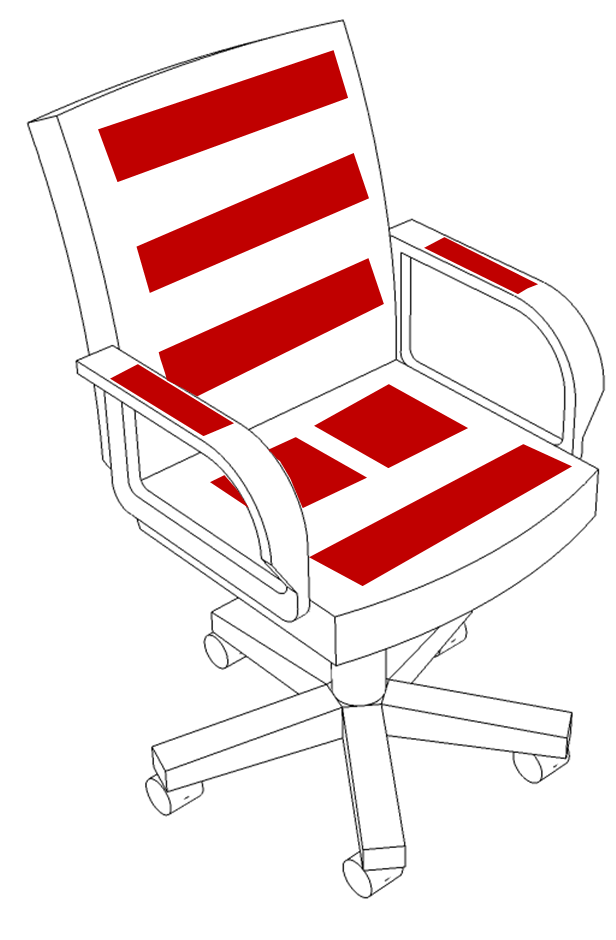
\includegraphics[width=0.4\textwidth]{images/smartofficechair}
\caption{Smart office chair sketch - eight electrodes three in backrest, three on seat and two in armrests}
\label{fig:smartchair_sketch}
\end{figure}
The Capacitive Chair is a regular office chair equipped with eight capacitive proximity sensors that can detect different sitting postures and work-related stress levels by examining movement and breathing rate \cite{Braun2013ChairAid}. Seven solid copper electrodes that are placed below the covering are augmented by a single conductive thread electrode that is placed in a mesh on the backrest. In the past smart chairs have used pressure sensors to infer posture and occupation \cite{tan2001sensing}. Combining presence and proximity sensing it is possible to directly infer postures where parts of the body do not touch the surface, e.g. if the body is arched towards the front, or if an arm is raised from the armrests. Additionally higher area electrodes in the backrest allow detecting the breathing rate by measuring the movement of the chest.

The Capacitive Chair aims at providing different services to a typical office worker and office managers. Using the occupation detection it is possible to advise for some type of physical activity, if the time spent in front of the screen was too long. The system can also advise the user to change to a more back-friendly posture or regularly switch the stance to achieve a more general workout. Using the breathing rate detection we are able to get some sort of measure of the current stress level associated to the given working situation. By adapting the environment it is possible to improve the working atmosphere and reduce stress. The Capacitive Chair uses a multifacetted data processing approach. A machine learning algorithm is associating the sensing data to one of nine different typical sitting positions, inspired by a recent study of sitting positions for modern device usage \cite{globalPosture}. An adaptive body model that is fitted to the current sensor values allows for fine grained adaptation of those postures. Finally a combination of Fourier and data variation analysis is calculating the current breathing rate \cite{Braun2013ChairAid}.

\subsubsection{Capacitive layout}
The Capacitive Chair is based on a single OpenCapSense board that supports eight different electrodes. In order to get the posture measurements we need to distribute the electrodes equally on the different areas of the seat. The measurement of the breathing rate requires a larger electrode near the chest area. Consequently the electrodes are placed as follows:
\begin{enumerate}
\item Electrode on the upper part of the backrest (covered by faux leather)
\item Electrode in the central part of the backrest (using conductive thread)
\item Electrode in the lower part of the backrest (covered by faux leather)
\item Electrode below the right armrest
\item Electrode below the left armrest
\item Electrode for the left hip area below the left part of the seat
\item Electrode for the right hip area below the right part of the seat
\item Electrode for detecting both legs below the front part of the seat
\end{enumerate}

\begin{minipage}{\linewidth}
\centering
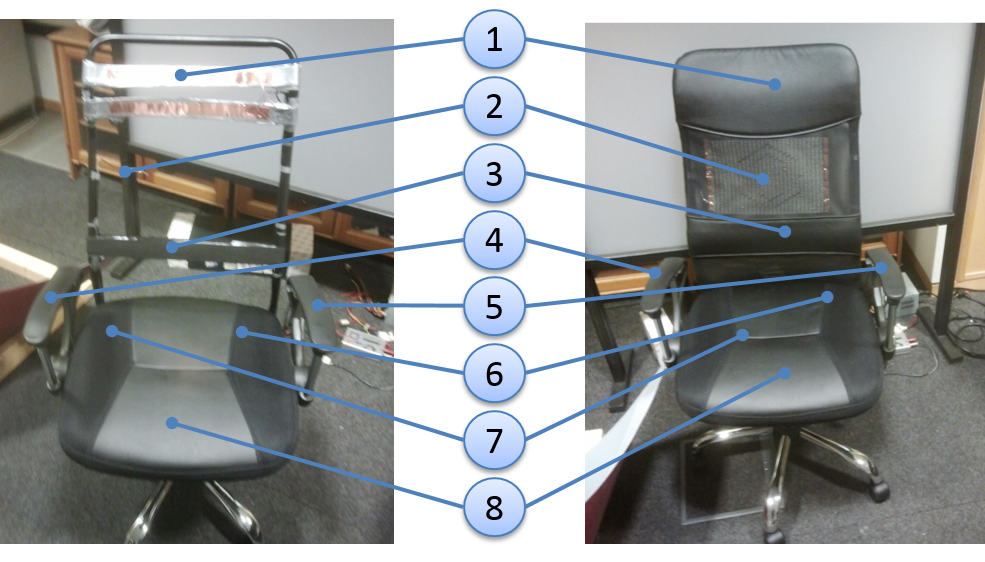
\includegraphics[width=0.8\textwidth]{images/prot_capchair_electrode_layout}
\captionof{figure}{Capacitive Chair electrode positions}
\label{fig:prot_capchair_electrode_layout}
\end{minipage}

The electrode is connected to channel 0 (CH0) of the OpenCapSense evaluation board. The following figure shows the layout of the electrode (2) including sensing electronics (5). The shield electrode is additionally the support structure for the whole setup here. The shield electrode is comprised of copper sheet bedded in duct tape. On the duct tape there are strips of copper sheet applied using conductive glue (2). The copper sheet is the sensing electrode connected to the sensor (5) using the blue wire (4). The shield electrode is connected using the red wire. The frame of the backrest is indicated using the number (6). 
This electrode in the lower part of the backrest is connected to CH2 of the OpenCapSense evaluation board.
The layout is analog to the one on the upper part of the backrest, comprised of shield electrode (2) covered by duct tape and a copper sheet electrode. The electrode on the right armrest is connected to CH3, the one on the left side to CH4 of the OpenCapSense evaluation board. Both electrodes are comprised of a copper sheet fixed to the armrest using duct tape. 
The electrode below the right hip area is connected to CH5, the one below the left hip area to CH6 and the leg electrode to CH7.
The figure above shows the electrodes. All of them are made of unprocessed, two-layer copper PCBs. They are isolated to the environment using duct tape. The electrode for the leg area is comprised of two distinct PCBs (2,3) that are connected using copper wire (5). The hip electrodes (1) are similarly comprised of copper PCBs. The wires are guided through the wooden seat using small drill holes (4,6). The red wire leads to the sensing electrode while the grey wire leads to the shielding.

\begin{minipage}{\linewidth}
\centering
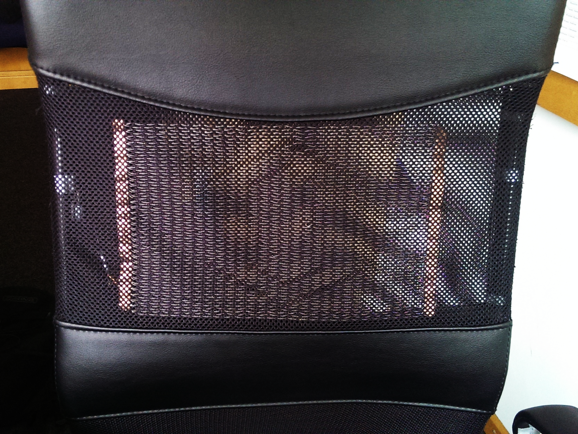
\includegraphics[width=0.8\textwidth]{images/prot_capchair_threadelectrode}
\captionof{figure}{Detail view of conductive thread electrode}
\label{fig:prot_capchair_threadelectrode}
\end{minipage}

The electrode in the central part of the backrest is connected to CH1 of the OpenCapsense evaluation board.
The electrode (1) is comprised of conductive thread that was woven into the covering of the backrest. The ends of the conductive thread are connected to a conductive copper foil. This foil is formed in such a way (4 left) that a terminal (4 right) can be applied and connected to the sensor electronics (3). This type of electrode does not support any shielding. In order to remove the covering the terminal should be disconnected from the electrode first.
 
\subsubsection{Processing}
The first step of data processing is filtering. We have implemented different types of filters, including static average and floating average filters. In this case we are using a median filter that is taking the median value of eight previous samples. After filtering we are building the baseline for each sensor channel. The baseline is the minimal sensor value that is created by sampling the environment without any object present. There is a plausibility check in this step to discard values that deviate too far from the norm. The maximum values of a channel are collected on run-time. Again we are using a plausibility check. The final step of pre-processing is a normalization based on acquired minimum and maximum values. For further processing we additionally need information about short-term value variance that we gather by calculating the difference quotient using a sample of ten average filtered measurements.
Afterwards we are performing a fast fourier transformation (FFT) to get information about the frequency spectrum of the sensor values, in order to perform breathing rate detection. 
\subsubsection*{Breathing rate detection} 
We are using the FFT values of sensors attached to the central backrest to get the current breathing rate. A binning operation is performed to look for significant signals in a reasonable frequency interval (0.1Hz-3Hz).
In order to increase the reliability of the breathing rate detection we use a second method. Based on the normalized values a mean value curve is calculated. The intersection points of this mean value curve and the current sensor values are additionally stored. We are using a dynamically weighted combination of both values to increase the reliability of the breathing rate detection.
\subsubsection*{Posture recognition, kinematics of the human body}
The processed values of all sensors are compared to previously trained sitting positions of a user. The position with the lowest deviation is considered the current posture. Currently the system supports nine different postures; however it can be dynamically extended or reduced.
Based on the normalized sensor values and geometric positions of the sensors the data is interpreted as position of the different joints of a user. 
4.2.4	Output
The GUI allows displaying of raw and processed data. In the following section we are presenting the different forms of interaction.
 
Figure 13 GUI with four opened windows
Figure 11 gives on overview of the GUI. Selecting the desired output in the ToolBox (1) opens the associated window. In this case we can see the data display of sensor channel 1 (2), the recognized breathing rate (4), the FFT of sensor channel 1 (3) and the recognized postures and their deviations (5).
 
Figure 14 GUI with two windows
Figure 12 shows two additional windows. On the left side (1) we can see a picture depicting the currently recognized posture; on the right side (2) we can see the human model with recognized joint positions. The 3D joint recognition is still in strong development and will be remodeled in the future.
Additional screens that have not been shown in this overview are a serial monitor that displays the raw data acquired from the USB connection, the collection of measurements using software queries, the display of all sensor values in table format and a repositioning of the different windows.
\subsubsection*{Distinguish work activity levels}
 
Figure 15 Work Activity aggregation over a single work day (mock-up)
Figure 13 shows a mock-up of a typical work day activity over a single work day. We assume the work day of a typical office worker and support three different aggregated activities: 
Active work as indicated by a certain level of movement while on the chair
Passive work as being present on the chair while not moving a lot
Not present at desk, whereas no one is currently sitting on the chair.


\subsubsection{Evaluation}
The Capacitive Chair was partially supported by the EIT ICT Labs project Cognitive Endurance during 2013. In this scope it was evaluated in two distinct studies. The first aimed at testing the aggregated recognition of working activities with several persons over various days. The second study was testing the posture recognition with various users that were additionally queried about their general impression of the system. In this section we are presenting results of both studies.
\subsubsection*{Working situation recognition}
The sensing chair supports distinguishing two different working situations that are determined using the method described in the previous section. The system also supports sending to the Cognitive Endurance server.
 
Figure \ref{fig:prot_capchair_eval_work} shows an example of this generated activity log. We have performed a test over 3 days between December 4th 2013 and December 6th 2013 on a typical work day in the office. The resulting activity logs were used to generate a chart as shown in the previous section. An example chart is shown in Figure 15.

\begin{minipage}{\linewidth}
\centering
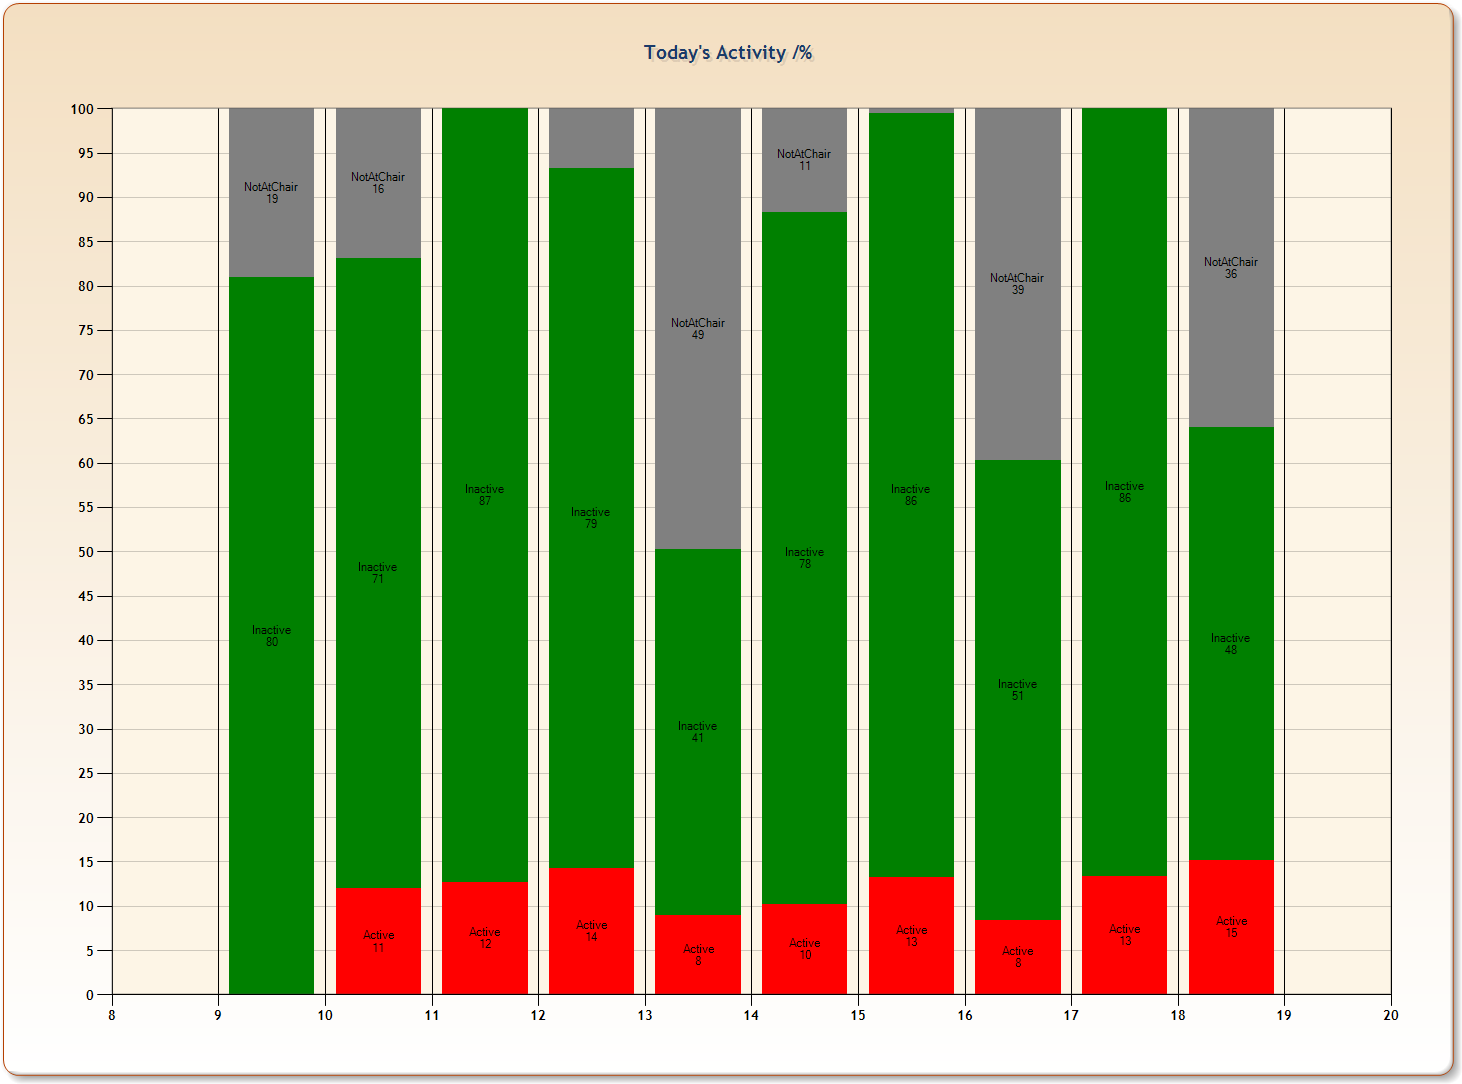
\includegraphics[width=0.8\textwidth]{images/prot_capchair_eval_work}
\captionof{figure}{Example chart of work activity data collected}
\label{fig:prot_capchair_eval_work}
\end{minipage}	

We can clearly see some phases of not at chair - usually for lunch break or some meetings and the work is distributed between active work, such as writing and typing and longer phases of inactivity (such as reading).

\subsubsection*{Posture recognition - test 1}
In a second evaluation we were testing the posture recognition of the chair in a short study with 10 participants. Our system was tuned to distinguish three poses and a non-pose:
\begin{itemize}
\item Sitting upright
\item Sitting hunched
\item “Slouching on chair”
\item Close to chair - disturber
\end{itemize}

The persons were given a short introduction, the different postures were displayed, and finally the persons were asked to perform the postures in order. When testing “close-to-chair” the subjects were asked to rattle at the chair, stand close, move it around and thus disturb the potential sensor readings. Each class was tested for 10 seconds, collecting 200 samples. Some impressions can be found in the following pictures:

\begin{minipage}{\linewidth}
\centering
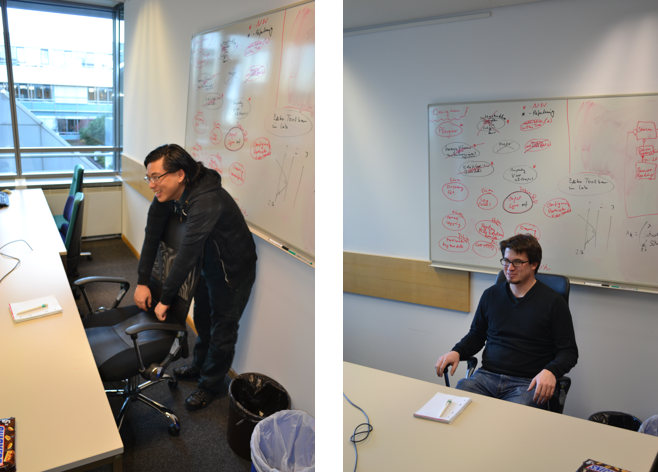
\includegraphics[width=0.8\textwidth]{images/prot_capchair_eval_pos1}
\captionof{figure}{Disturber position of a participant (left) and sitting upright (right)}
\label{fig:prot_capchair_eval_pos1}
\end{minipage}	 

\begin{minipage}{\linewidth}
\centering
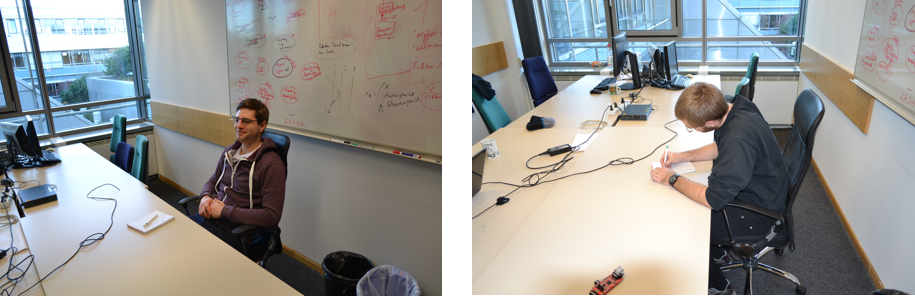
\includegraphics[width=0.8\textwidth]{images/prot_capchair_eval_pos2}
\captionof{figure}{Slouching position (left) and sitting hunched (right)}
\label{fig:prot_capchair_eval_pos2}
\end{minipage}

Overall the results were very convincing. Of the 40 different measurements series only two were not achieving 100\% accuracy. The Upright and Disturbance positions were classified correctly for all candidates. A single candidate had an 86\% rating on the hunched posture. A different candidate had a 55\% rating on the slouching position. The average of correctly classified postures is 98,5\%.


